% Commented out: 
% \addbibresource
% \includepdf

\documentclass[12pt,letterpaper,english,bibliography=totocnumbered, abstract=on]{scrartcl}

\usepackage{indentfirst}
\usepackage[titletoc]{appendix}
%\usepackage{fullpage}
%\usepackage{subfiles}
\usepackage[T1]{fontenc}
\usepackage[latin9]{inputenc}
\usepackage{color}
\usepackage{babel}
\usepackage{verbatim}
\usepackage[unicode=true,pdfusetitle,
bookmarks=true,bookmarksnumbered=false,bookmarksopen=false,
breaklinks=true,pdfborder={0 0 0},pdfborderstyle={},backref=false,colorlinks=true]
{hyperref}
\hypersetup{linkcolor=blue,citecolor=blue,urlcolor=blue}

\usepackage{booktabs}
\usepackage{multirow}
\usepackage{adjustbox}
\usepackage{threeparttable}
\usepackage[table]{xcolor}
\usepackage{csquotes}
\usepackage{soul} % for hiliting text: \hl

\usepackage[backend=biber, style=authoryear, maxbibnames=99, dashed=false]{biblatex}
\setlength\bibitemsep{2\itemsep}
\addbibresource{refs.bib}

\usepackage{pdfpages}
\usepackage{float} % Allows use of H to place floats

\usepackage{pgfgantt}

\usepackage{framed}

\usepackage{subcaption}

% Prevent page breaks within paragraphs
% https://tex.stackexchange.com/questions/21983/how-to-avoid-page-breaks-inside-paragraphs
\widowpenalties 1 10000

% The following package automatically provides ragged right formatting for text within table cells.
\usepackage[raggedrightboxes]{ragged2e}

\begin{document}

\titlehead{DRAFT}

\title{First Record of Nematodes Associated with Coconut Rhinoceros Beetle, \textit{Oryctes rhinoceros}, on Guam}

\author{Aubrey Moore and Laura Caser \\ University of Guam}

%\date{May 5, 2020\\Revised May 4, 2021}

\maketitle
%\footnote{\url{https://github.com/aubreymoore/2020-FS-CRB-biocontrol-project/blob/master/combined-proposal.pdf}}
%\newpage
%\tableofcontents

%\pagebreak

Coconut rhinoceros beetle (CRB), \textit{Oryctes rhinoceros} (Scarabaeidae: Dynastinae), was first detected on Guam during 2007, quickly spread throughout the island and has killed many coconut palms \parencite{marshall_new_2017-1}.
We are performing laboratory bioassays of several \textit{Oryctes rhinoceros} nudivirus OrNV isolates in an attempt to find effective biological control agent candidates for the virus-resistant CRB biotype we are trying to control on Guam. 

On August 14, 2023 while doing postmortem examinations of adult beetles which died in these assays, we detected nematodes on the dorsal surface of the abdomen of a dead beetle. \href{https://www.youtube.com/shorts/dKVup7q7FF0}{Click here} to see a YouTube video of the original discovery.

Since then, we have observed that 55\% (65 of 110 dead or dying adult beetles from the bioassays) have been infested with nematodes (Fig. \ref{fig:nematode}). Most of the time, these are observed underneath the elytra or on the ventral surface of the abdomen. Numbers range from a few to hundreds of nematodes per beetle. On several occasions, nematodes were observed swimming within the hemocoel.

We currently seek help to identify these nematodes.

% TODO: \usepackage{graphicx} required
\begin{figure}[H]
	\centering
	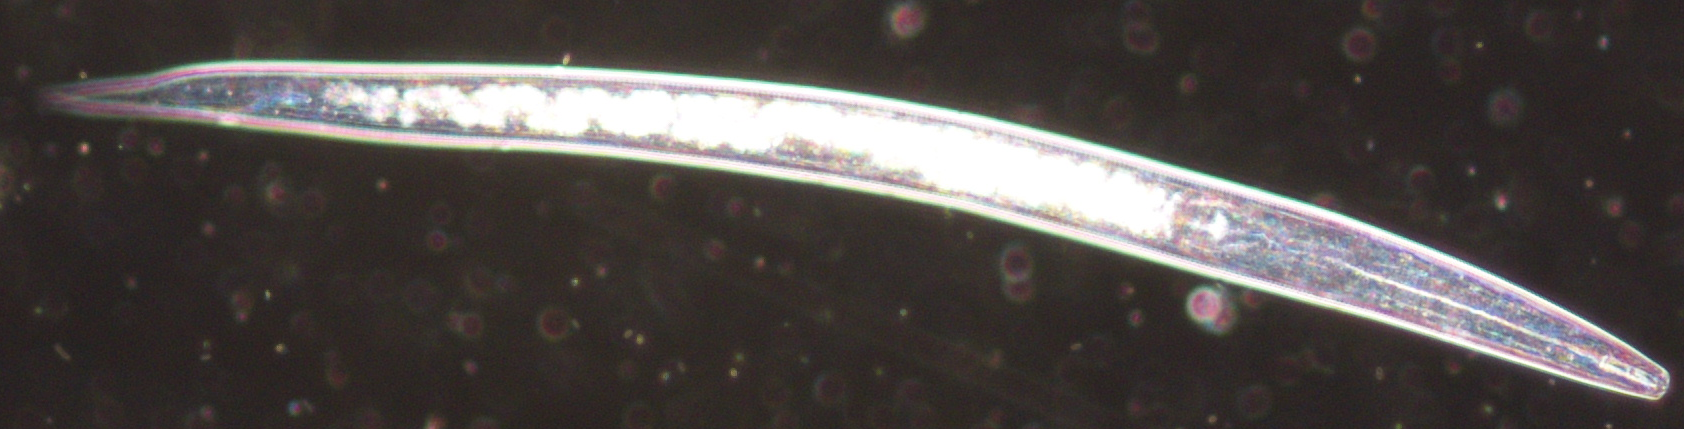
\includegraphics[width=\linewidth]{images/nematode2}
	\caption{Nematode collected from beneath elytra of an adult coconut rhinoceros beetle, \textit{Oryctes rhinoceros}. Length is 0.36 mm.}
	\label{fig:nematode}
\end{figure}

%
%\begin{figure}[H]
%	\centering
%	\begin{subfigure}{.5\textwidth}
%		\centering
%		\includegraphics[width=\linewidth]{images/bioassay1}
%		\caption{Droplet dosing method}
%		\label{fig:sub1}
%	\end{subfigure}%
%	\begin{subfigure}{.5\textwidth}
%		\centering
%		\includegraphics[width=\linewidth]{images/bioassay2}
%		\caption{Tube dosing method}
%		\label{fig:sub2}
%	\end{subfigure}
%	\caption{Black horizontal lines indicate mass containing 5,000 infective units (UI) of OrNV. This level is the the minimum dose recommended to establish infection in a susceptible beetle \parencite{AgResearch2023}.}
%	\label{fig:paired-plots}
%\end{figure}
%
%
%\section{Notes}
%
%\begin{enumerate}
%	\item Our technique might work better if we increase sugar content (currently 5\%). Sugar content of coconut sap is 12.92\% (6.91\% sucrose, 3.48\% fructose, and 2.53\% glucose) (\cite{asgharCoconutCocosNucifera2019}).	
%\end{enumerate}


\printbibliography

\end{document}
